\chapter{MHD equilibrium problem}\label{chapter:GS}
In this chapter, after a short introduction where we summarize what is a plasma and the differences way to confine it, we focus our attention to the mirror machine, which is a particular configurations for confinement, describing the physical principle behind that: the conservation of magnetic moment. Finally, starting from a fluid model, we derive the equilibrium equation for a plasma confined by the mirror device.

\section{Introduction}\label{sec:introduction}
Plasma is one of the four fundamental states of matter which consists in an ionized gas. More precisely it is a high-temperature collection of independently moving charged particles, ions and electrons, dominated by electromagnetic forces. Ionization can be induced by heating a gas or by strong electromagnetic field applied with a laser or microwave generator. The presence of a non-negligible number of charge carriers makes the plasma electrically conductive so that it responds strongly to electromagnetic fields. The motion depends not only on local conditions, but on the state of plasma in remote regions as well, because elements of plasma exert a force on one another even at large distances. In fact the motion of local concentrations of charged particles, which give rise to electric field, generates currents and thence a magnetic field that affects the motion of other particles. Cmp. \cite{CHEN}.
\medskip

Criteria for plasma:
\begin{itemize}
  \item $\lambda_D\ll L$ When the Debye length, defined as $\lambda_D=\sqrt{\frac{\epsilon_0 k_B T_e}{n_eq_e^2}}$ is short compared to the physical size L of the plasma, then the plasma is quasineutral. Quasineutral means that the ionized gas is neutral enough so that globally the density of ions is approximatively equals to the density of electrons $n_i\simeq n_e\simeq n$ but locally no so neutral that all the interesting forces vanish. This criterion sets the predominance of interactions in the bulk of plasma over those at its edges, where boundary effects may take place.
  \item $N_D\ll 1$ The plasma approximation is valid when the number of charge carriers within the Debye sphere of influence $N_D=n\frac{4}{3}\pi\lambda_D^3$ of a particular particle is higher than unity to provide collective behavior of the charged particles.
  \item $\omega_{\tau}>1$ When the frequency $\omega$ of typical plasma oscillations is large than the frequency $\frac{1}{\tau}$ of collision with neutral atoms, then electrostatic interactions dominate over the processes of ordinary gas kinetics.
\end{itemize}

Fusion is a form of nuclear energy which consists in the merging of light elements, mainly hydrogen (H) and its isotopes deuterium (D) and tritium (T) to produce energy. To burn D–T one is required to heat it to the astounding temperature of $1.5\cdot 10^6 K$, hotter than the center of the sun. Once heated some method must be devised to hold the plasma together. The primary method requires a clever configuration of magnetic fields.
\medskip

The determination of MHD equilibrium configurations is an integral part of the problem of designing plasma confinement devices. Indeed equilibrium calculations play a major role in reactor studies where a knowledge of the plasma configuration provides the basic framework for detailed system design. The Grad-Shafranov equation is a two dimensional, nonlinear elliptic PDE which describes the relation between the plasma current and the pressure in terms of flux. It provides a complete description of ideal MHD equilibrium.
\medskip

At present, there are two main types of magnetic configurations for plasma confinement: closed (tokamak, stellarator, etc) and open (mirrors). Although closed configurations are more developed, advantages of the open systems could be useful in future for the fusion program. It should be mentioned the most important features of open systems:
\begin{itemize}
  \item most of such systems can operate in steady state regime and, at the same time, effects of disruptions are not appeared in them;
  \item plasma pressure can be comparable with magnetic field pressure;
  \item there are no divertor problems in the mirror case;
  \item open systems are convenient for direct energy conversion of charged particles. This circumstance can turn out to be especially important in a future for low-neutron schemes of fusion reactions.
\end{itemize}

\section{The mirror machine}\label{sec:mirror_machine}
The simplest device designed to confined a plasma is the mirror machine: it leverages the mirror effect to trap plasma particles using magnetic fields. To understand how it works it is necessary to briefly summarize the theory known as \textit{Single-particle motion} which describes the motion of charged of charged particles in prescribed magnetic and electric fields. For a more detailed explanation cmp. \cite{plasma}.

The starting point are the equations of motion as determined from Newton’s law. For plasma physics applications, only the magnetic and electric forces, given by Lorentz force, are required since gravity has a very small effect and can be neglected. The equations to be solved are thus:
\begin{equation}\label{eq:newton}
  \begin{cases}
    m\frac{\mathrm{d}\mathbf{v}}{\mathrm{d}t}=q(\mathbf{E}+\textbf{v}\times{\mathbf{B}})\\
    \frac{\mathrm{d}\mathbf{r}}{\mathrm{d}t}=\mathbf{v}
  \end{cases}
\end{equation}
where $\mathbf{B}=\mathbf{B}(\mathbf{r},t)$ and $\mathbf{E}=\mathbf{E}(\mathbf{r},t)$. The fields are simply specified as known quantities, therefore self-consistency is not taken in account. $\textbf{B}$ and $\textbf{E}$ are assumed to be smooth, slowly varying functions in order to be compatible with the requirement that plasmas be dominated by long-range collective effects.

It is possible to study the motion of a single particle using specific configurations of the two fields in order to solve analytically the model (\ref{eq:newton}); combining all the motions, the general trajectory of a particle is obtained. The mirroring takes place when one of these specific configurations is used.
\medskip

Let's suppose to have the following fields
\begin{equation}\label{eq:fields_magnetic_moment}
  \begin{cases}
    \mathbf{E}_{\perp}=E_x(x,t)\mathbf{e}_y\\
    \mathbf{B}=B(t)\mathbf{e}_z.
  \end{cases}
\end{equation}
Substituting Eq.(\ref{eq:fields_magnetic_moment}) in Eq.(\ref{eq:newton}) it is possible to derive, using some physical considerations, the following simplified system
\begin{equation}\label{eq:newton_simp}
  \begin{cases}
    \frac{\mathrm{d}v_x}{\mathrm{d}t}-\omega_cv_y=0\\
    \frac{\mathrm{d}v_y}{\mathrm{d}t}+\omega_cv_x=\frac{\omega_c}{B}\big(E_y+\frac{\partial E_y}{\partial x_g}(x-x_g)\big)
  \end{cases}
\end{equation}
where $\omega_c=\frac{qB}{m}$ is the gyro frequency and $(x_g,y_g)$ is the center, called guiding center, of the orbit of the circular-type motion described by the charged particle in the prescribed field. The right-hand side of the second equation (\ref{eq:newton_simp}) is a first order expansion around the guiding center. Introducing a new time variable
\begin{equation}
  \tau=\int_0^t\omega_c(t')\:\mathrm{d}t',
\end{equation}
which implies $\mathrm{d}\tau=\omega_c\mathrm{d}t$, we can reduce the model to
\begin{equation}\label{eq:newton_simp_bis}
  \begin{cases}
    \frac{\mathrm{d}v_x}{\mathrm{d}\tau}-v_y=0\\
    \frac{\mathrm{d}v_y}{\mathrm{d}\tau}+v_x=\frac{1}{B}\big(E_y+\frac{\partial E_y}{\partial x_g}(x-x_g)\big)\\
    \frac{{d}x}{\mathrm{d}\tau}=\frac{v_x}{\omega_c}\\
    \frac{{d}y}{\mathrm{d}\tau}=\frac{v_y}{\omega_c}.
  \end{cases}
\end{equation}
We can rewrite $v_x$ and $v_y$ in terms cylindrical velocity coordinates:
\begin{equation}\label{eq:cylindrical_velocities}
  \begin{cases}
    v_x=v_{\perp}(\tau)\cos(\tau+\varepsilon(\tau))+\frac{E_y}{B}\\
    v_y=-v_{\perp}(\tau)\sin(\tau+\varepsilon(\tau))+\frac{\mathrm{d}}{\mathrm{d}\tau}\big(\frac{E_y}{B}\big)
  \end{cases}
\end{equation}
where the variables $v_x$ and $v_y$ have been replaced by new unknowns $v_{\perp}(\tau)$, $\varepsilon(\tau)$. The remainder of the analysis focuses on solving $v_{\perp}(\tau)$ since it gives origin to an approximate constant of the motion. The solution for $\varepsilon(\tau)$ can also be easily found but no new important information is contained therein and hence the corresponding analysis is suppressed. Before substituting Eq.(\ref{eq:cylindrical_velocities}) in Eq.(\ref{eq:newton_simp_bis}) it is necessary to find an expression for the term $x-x_g$; since this expression appears only in the small, expanded term, the leading order gyro motion contribution is all that is required. From the second two trajectory equations in Eq.(\ref{eq:newton_simp_bis}) one finds that
\begin{equation}\label{eq:approx_gyro_coor}
  x-x_g\approx\frac{v_{\perp}(\tau)}{\omega_c(\tau)}\sin(\tau+\varepsilon(\tau)).
\end{equation}
Substituting Eq.(\ref{eq:approx_gyro_coor}) and Eq.(\ref{eq:cylindrical_velocities}) in Eq.(\ref{eq:newton_simp_bis}), solving simultaneously for $\frac{\mathrm{d}v_{\perp}}{\mathrm{d}\tau}$, $\frac{\mathrm{d}\varepsilon}{\mathrm{d}\tau}$ and using Faraday's law $\frac{\partial E_y}{\partial x_g}=-\frac{\mathrm{d}B}{\mathrm{d}t}=-\omega_c\frac{\mathrm{d}B}{\mathrm{d}\tau}$ it is possible to obtain
\begin{equation}\label{eq:magnetic_moment}
  \frac{1}{\mu}\frac{\mathrm{d}\mu}{\mathrm{d}\tau}=\frac{1}{B}\frac{\mathrm{d}B}{\mathrm{d}\tau}\cos 2(\tau+\varepsilon)
\end{equation}
where
\begin{equation}
  \mu=\frac{mv^2_{\perp}}{2B};
\end{equation}
higher order terms have been neglected. The quantity $\mu$ is called \textit{magnetic moment}.
\medskip

The equation (\ref{eq:magnetic_moment}) can be further simplified integrating over one gyro period $\tau_0\leq\tau +\varepsilon\leq(\tau_0+2\pi)$. Indeed one finds that the right hand side almost exactly averages to zero, except for a very small, negligible correction. It follows that $\mu$ is a constant of the motion when averaged over one gyro period since
\begin{equation}
  \langle\frac{\mathrm{d}\ln\mu}{\mathrm{d}\tau}\rangle\approx0\qquad\Longrightarrow\qquad \mu=\mathrm{const}.
\end{equation}
The quantity $\mu$ is  also known as the first adiabatic invariant and is equal to the gyro-averaged magnetic moment of the charged particle. The fact that $\mu$ is constant when averaged over a gyro period can be interpreted as follows. The magnetic flux enclosed by a particle over one gyro orbit is just $\psi=\pi r^2B=\frac{2\pi m}{q^2}\mu\approx\mu$. Therefore, as the B field changes slowly in time the perpendicular velocity and corresponding gyro radius also change slowly in time in such a way that the flux contained within the orbit is a constant.

\begin{figure}
\centering
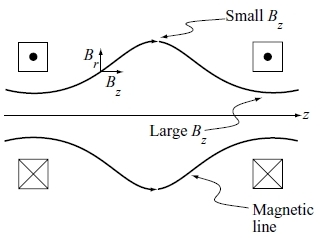
\includegraphics[scale=.6]{images/B_gradient.jpg}
\caption{Coil configuration generating a magnetic field gradient along $z$ direction.}
\label{fig:B_gradient}
\end{figure}

With an approach similar to the one followed before, we can study the effect of a parallel gradient in the magnetic field, which can arise in configurations such as those illustrated in  Fig.(\ref{fig:B_gradient}).The fields configuration in this case is
\begin{equation}\label{eq:fields_mirroring}
  \begin{cases}
    \mathbf{E}=0\\
    \mathbf{B}=B_x(x,z)\mathbf{e}_x+B_z(x,z)\mathbf{e}_z
  \end{cases}
\end{equation}
where, for simplicity, the geometry, Fig.(\ref{fig:B_gradient_slab}), is a slab version of the cylindrical configuration shown in Fig.(\ref{fig:B_gradient}).

\begin{figure}
\centering
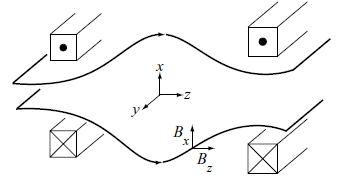
\includegraphics[scale=.6]{images/B_gradient_slab.jpg}
\caption{Slab approximation.}
\label{fig:B_gradient_slab}
\end{figure}

Two important results can be derived in the limit where the gyro radius is small compared to the spatial gradient length of the field. Firstly, the magnetic moment is again an adiabatic invariant but now the time dependency becomes a spatial since, after averaging over a gyro-period, $v_{\perp}=v_{\perp}(z)$ and $B=B(z)$. Secondly, it is possible to find gyro-averaged force acting on the parallel guiding center motion of the particle. The force is driven by the parallel gradient in the magnetic field and has the following expression
\begin{equation}
  m\frac{\mathrm{d}v_{\|}}{\mathrm{d}t}=-\mu\nabla_{\|}B.
\end{equation}

The combination of $\mu=\mathrm{const}$ and $F_{\|}=−\mu\nabla_{\|} B$ can rule the parallel motion of the guiding center. In particular, the direction of the parallel motion can be completely reversed since there is a critical point, called \textit{mirror point}, along the trajectory where the particle is reflected. This reversal process is named \textit{mirror effect}. This process is well described in Fig.(\ref{fig:mirroring}).

\begin{figure}
\centering
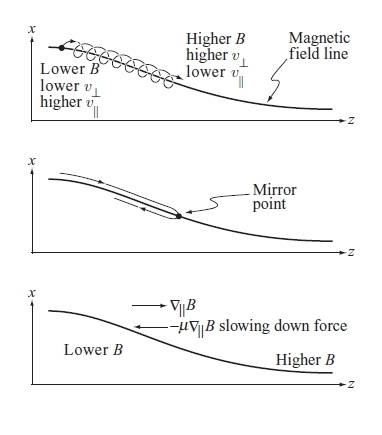
\includegraphics[scale=.6]{images/mirroring.jpg}
\caption{The mirror effect.}
\label{fig:mirroring}
\end{figure}

A particle, with initial velocity $(v_{\|},v_{\perp})$ moves from a region of lower field into the high-field region and the value of $B$ along the guiding center increases. Since $\mu=\frac{mv^2_{\perp}}{2B}=\mathrm{const}$, $v_{\perp}$ must increase and, since in a static magnetic field the kinetic energy of a particle is constant $E=\frac{1}{2}m(v_{\perp}^2+v_{\|}^2)=\mathrm{const}$, $v_{\|}$ must decrease. Therefore, if $B$ increases sufficiently, the particle reaches a point along its trajectory where $v_{\|}=0$: the reflection point. Once reflected, the parallel velocity of the particle reverses direction and the guiding center motion starts moving to the left. The force causing this behavior is $F_{\|}$.

\begin{figure}
\centering
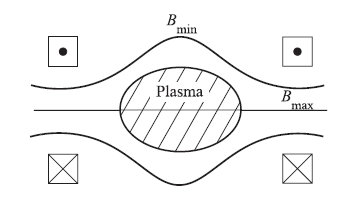
\includegraphics[scale=.6]{images/mirror_machine.jpg}
\caption{Geometry of the simplest mirror machine.}
\label{fig:mirror_machine}
\end{figure}

The mirror effect is the physical principle used to confine plasma in the earliest magnetic fusion configurations: the \textit{mirror machine}, cmp. Fig.(\ref{fig:mirror_machine}). This device simply consists of two coils with currents flowing in the same direction which create a magnetic field with a maximum just under each coil and a local minimum midway between. Using the guiding center theory, it is simple to evaluate that a large fraction of the particles remain confined. Unfortunately practical experiments have shown that the simple mirror machine did not work as well as predicted since macroscopic and microscopic instabilities were observed, leading to anomalously fast losses of particles at the extreme points of the device. Indeed Coulomb collisions scatter many particles to very high parallel velocity and these particles escape from the device.

\section{Grad-Shavranov equation}\label{sec:grad_shavranov}
The densities of plasmas are such that they belong to an intermediate range between fluids and a collection of individual particles. Under appropriate hypothesis the identity of individual particle is negligible and only the motion of conducting fluids is taken into account, so we can study the plasma confinement in the mirror machine within the ideal magnetohydrodynamics (MHD) which is a single-fluid model. The MHD model is a reduction of the two-fluid model, where ions and electrons are described like two fluids by conservation equations coupled with Maxwell's equations, derived by focusing attention on the length and time scales characteristic of macroscopic behavior. For more details cmp. \cite{GUO}, \cite{plasma} and \cite{idealMHD}. The explicit computations are reported in Appendix.
\medskip

The MHD equilibrium model is
\begin{subequations}\label{eq:MHD_equlibrium}
  \begin{align}
    \label{eq:MHD_momentum}\mathbf{J}\times\mathbf{B}&=\nabla\cdot\mathbb{P}\\
    \label{eq:MHD_current}\nabla\times\mathbf{B}&=\mathbf{J}\\
    \label{eq:MHD_maxwell}\nabla\cdot\mathbf{B}&=0
  \end{align}
\end{subequations}
where $\mathbf{B}$ is the magnetic field, $\mathbf{J}$ is the plasma current and $\mathbb{P}$ is the gyrotropic pressure tensor defined as
\begin{equation}\label{eq:pressure_tensor}
  \mathbb{P}=p_\perp\mathbb{I}+(p_\parallel - p_\perp)\mathbf{b}\otimes\mathbf{b}.
\end{equation}

The vector $\mathbf{b}=\frac{\mathbf{B}}{B}$ is the unit vector parallel to $\mathbf{B}$ and $B=\|\mathbf{B}\|$ is the magnitude of the magnetic field; the scalar components $p_\perp$ and $p_\parallel$ are definable in terms of a distribution function $g_0$ of guiding centers , cmp. \cite[p. 1614]{magnetic_mirror}, as
\begin{equation}\label{eq:pressure_components}
  p_\perp=\int g_0\,v^2_\perp \mathrm{d}^3 v \quad\mbox{and}\quad p_\parallel=\int g_0\,v^2_\parallel \mathrm{d}^3 v
\end{equation}
where $v_\perp$ and $v_\parallel$ are the component of fluid velocity perpendicular and parallel to the magnetic field, respectively, and
$\mathrm{d}^3 v=\mathrm{d}v_\perp\mathrm{d}v_\parallel\mathrm{d}\phi$.

Equation (\ref{eq:MHD_current}) is the Ampere law while (\ref{eq:MHD_maxwell}) represents the conservation of magnetic flow; equation (\ref{eq:MHD_momentum}) establishes that at the equilibrium there is a balance force between force due to the pressure and Lorentz force $\mathbf{J}\times\mathbf{B}$.
\medskip

Taking the divergence of (\ref{eq:pressure_tensor}) and introducing the magnetic field-line curvature vector $\mathbf{k}=\mathbf{b}\cdot\nabla\mathbf{b}=(\nabla\times\mathbf{b})\times\mathbf{b}$, we obtain
\begin{equation}\label{eq:div_press}
  \nabla\cdot\mathbb{P}=\nabla p_\perp+(p_\parallel - p_\perp)\mathbf{k}+\left[\mathbf{b}\cdot\nabla(p_\parallel - p_\perp)-
  \frac{1}{B}(p_\parallel - p_\perp)\nabla B\cdot\mathbf{b}\right]\mathbf{b}
\end{equation}
  and taking the dot product between (\ref{eq:div_press}) and $\mathbf{b}$, we find the relation between $p_\perp$ and $p_\parallel$ along the magnetic field
\begin{equation}\label{eq:pressure_balance}
  p_\perp=p_\parallel-B\frac{\partial p_\parallel}{\partial B}.
\end{equation}

This relation replaces the simple condition $\mathbf{b}\cdot\nabla p=0$ of the isotropic scalar pressure theory. The longitudinal pressure balance equation states that only if $p_\perp>p_\parallel$ it is possible to balance the plasma pressure $p_\parallel$ using a positive gradient of $\mathbf{B}$.

Moreover we can find the expression for the parallel and perpendicular components of the plasma current respect to the magnetic field. From Eq.(\ref{eq:MHD_momentum}) we have
\begin{equation}
  \mathbf{B}\times\mathbf{J}\times\mathbf{B}=\mathbf{B}\times\nabla\cdot\mathbb{P}
\end{equation}
but
\begin{equation}
  \mathbf{B}\times\mathbf{J}\times\mathbf{B}=(\mathbf{B}\cdot\mathbf{B})\mathbf{J}-(\mathbf{B}\cdot\mathbf{J})\mathbf{B}=B^2\mathbf{J}-(\mathbf{B}\cdot\mathbf{J})\mathbf{B}
\end{equation}
so
\begin{equation}\label{eq:current_comp}
  \mathbf{J}=\frac{1}{B^2}(\mathbf{B}\cdot\mathbf{J})\mathbf{B}+\frac{1}{B^2}\mathbf{B}\times\nabla\cdot\mathbb{P}=
  (\mathbf{b}\cdot\mathbf{J})\mathbf{b}+\frac{1}{B}\mathbf{b}\times\nabla\cdot\mathbb{P}=\mathbf{J}_\parallel+\mathbf{J}_\perp
\end{equation}
\medskip

It is convenient to rewrite the system of equations (\ref{eq:MHD_equlibrium}) using the Clebsch coordinates $(\psi,\theta,\phi)$ or flux coordinates, cmp. \cite{fluxcoord}. To do that, firstly we define flux surface a smooth surface $S$ with normal $\textbf{n}$ such that $\mathbf{B}\cdot\mathbf{n}=0$ everywhere on $S$ which implies that the magnetic field does not cross $S$ anywhere.  It is then possible to define a scalar flux function $\psi$ such that its value is constant on $S$, and $\mathbf{B}\cdot\nabla \psi=0$. Assuming the flux surfaces have a toroidal topology, the function $\psi$ defines a set of nested surfaces, so it makes sense to use this function to label the flux surfaces, i.e., $\psi$ may be used as a "radial" coordinate. Each toroidal surface $\psi$ encloses a volume $V(\psi)$ and the surface corresponding to an infinitesimal volume is essentially a line which corresponds to the toroidal axis.

From (\ref{eq:MHD_maxwell}) it follows that $\mathbf{B}$ can be rewritten as
\begin{equation}
  \mathbf{B}=\nabla\times\mathbf{A}=\nabla\times(\alpha\nabla\beta)=\nabla\alpha\times\nabla\beta.
\end{equation}
The flux of $\mathbf{B}$ through a surface $S$ with unit normal vector $\mathbf{n}$ outward from the volume $V$, enclosed by $S$, is
\begin{equation}
  \int_S\mathbf{B}\cdot\mathrm{d}\mathbf{S}=\int_S(\nabla\times(\alpha\nabla\beta))\cdot\mathrm{d}\mathbf{S}=\oint_l\alpha\nabla\beta\cdot\mathrm{d}\mathbf{l}=\oint_l \alpha\mathrm{d}\beta;
\end{equation}
choosing $\alpha=\psi$ and $\beta=\theta$ we obtain
\begin{equation}\label{eq:clebsch}
  \mathbf{B}=\nabla\psi\times\nabla\theta
\end{equation}
end
\begin{equation}
 \int_S\mathbf{B}\cdot\mathrm{d}\mathbf{S}=\int_0^{2\pi} \psi\mathrm{d}\theta=2\pi\psi.
\end{equation}

Therefore, except for a proportionality constant, the coordinate $\psi$ measures the total magnetic flux enclosed within a constant $\psi$ surface. Instead $\theta$ is orthogonal to $\psi$ and it is $2\pi$-periodic angle-like on each flux surface. Finally let's call $\phi$ the distance along a field line, cmp. \cite[p. 1617]{magnetic_mirror}. Moreover $\mathbf{b}\cdot\nabla\psi=0$ and $\mathbf{b}\cdot\nabla\theta=0$ which means that $\psi$ and $\theta$ remain constant along field lines, but its value may vary from one filed line to another. In particular $\psi=\mathrm{const}$ define the axial flux surfaces upon which the trapped particle guiding centers move: it can be used to plot the trajectories of particles in the steady flow.
\medskip

Using the Clebsch coordinates it is possible to rewrite the system of equation (\ref{eq:MHD_equlibrium}) like an unique equilibrium equation in that reference frame but, for our purposes, it is better to choose a cylindric coordinates set $(r,\theta, z)$. Under the axisymmetric hypothesis, which means that $z$ is an axis of revolution and $\frac{\partial(\cdot)}{\partial \theta}=0$, the magnetic field is independent of the angular coordinate $\theta$. So $\psi=\psi(r,z)$ and its gradient can be written as
\begin{equation}
  \nabla\psi=\frac{\partial\psi}{\partial r}\nabla r+\frac{\partial\psi}{\partial z}\nabla z
\end{equation}
and (\ref{eq:clebsch}) becomes
\begin{equation}
  \mathbf{B}= \frac{\partial\psi}{\partial r}\nabla r \times\nabla\theta+\frac{\partial\psi}{\partial z}\nabla z \times\nabla\theta
\end{equation}
or in the covariant basis $(\mathbf{e}_r,\mathbf{e}_\theta,\mathbf{e}_z)$, where $\mathbf{e}_\theta=r\nabla\theta$,
\begin{equation}\label{eq:covariantB}
 \mathbf{B}=-\frac{1}{r}\frac{\partial\psi}{\partial z}\mathbf{e}_r+\frac{1}{r}\frac{\partial\psi}{\partial r}\mathbf{e}_z.
\end{equation}

From (\ref{eq:covariantB}) and (\ref{eq:MHD_current}) we obtain the current in contravariant components
\begin{equation}\label{eq:covJ}
  \mathbf{J}=-\left[\frac{\partial}{\partial r} \left(\frac{1}{r} \frac{\partial \psi}{\partial r}\right) + \frac{1}{r} \frac{\partial^2 \psi}{\partial z^2}\right]\mathbf{e}_\theta=
  -r\left[\frac{\partial}{\partial r} \left(\frac{1}{r} \frac{\partial \psi}{\partial r}\right) + \frac{1}{r} \frac{\partial^2 \psi}{\partial z^2}\right]\nabla\theta
\end{equation}
and, since it holds (\ref{eq:current_comp}), we can decompose it as
\begin{subequations}\label{eq:plasma_current}
  \begin{align}
    \mathbf{J}_\parallel=0\\
    \label{eq:perp_curr}\mathbf{J}_\perp=\frac{1}{1+\eta}\bigg[\mathbf{B}\times\nabla\eta+\frac{1}{B^2}\frac{\partial p_\parallel}{\partial \psi}\mathbf{B}\times\nabla\psi\bigg],
  \end{align}
\end{subequations}
which implies that $\mathbf{J}=\mathbf{J}_\perp$.

Equating (\ref{eq:perp_curr}) with (\ref{eq:covJ}) and using (\ref{eq:clebsch}) and the fact that $|\nabla\psi|=rB$ we obtain
\begin{equation}\label{eq:GS_operator}
 -\Delta^*\psi=\frac{1}{1+\eta}\bigg[\nabla\eta\cdot\nabla\psi+r^2\frac{\partial p_\parallel}{\partial \psi}\bigg]
\end{equation}
where
\begin{equation}
  \eta=\frac{1}{B^2}(p_\perp-p_\parallel)=-\frac{1}{B}\frac{\partial p_\parallel}{\partial B}
\end{equation}
 and $\Delta^*$ is the linear elliptic operator defined as
\begin{equation}
  \Delta^*f=r\nabla\cdot\left(\frac{\nabla f}{r}\right)=r\frac{\partial }{\partial r} \left(\frac{1}{r} \frac{\partial f}{\partial r}\right) + \frac{\partial^2 f}{\partial z^2}=
  \Delta f -\frac{2}{r}\frac{\partial f}{\partial r}.
\end{equation}

The Grad-Shafranov equilibrium problem for the simple mirror in the anisotropic case under the axisymmetric hypothesis assumes the following formulation
\begin{equation}\label{eq:GS_eq}
  -\Delta^*\psi=\frac{1}{1-B^{-1}\partial p_\parallel/\partial B}\bigg[-\nabla \Big(B^{-1}\frac{\partial p_\parallel}{\partial B}\Big)\cdot\nabla\psi+
  r^2\frac{\partial p_\parallel}{\partial \psi}\bigg].
\end{equation}

The problem can be solved when we prescribe the parallel pressure profile $p_\parallel(\psi,B)$. It is now possible determine the spatial distribution of the plasma and the field, and then to calculate in detail the magnetostatic equilibria for the mirror.
\medskip

The equilibrium equation (\ref{eq:GS_eq}) involves two differentiation operators $\nabla$ and $\partial/\partial\psi$, so two kinds of formulations are possible.

The first one, referred as \textit{direct problem}, consist to solve (\ref{eq:GS_eq}) in the real space $(r,z)$ and find the solution $\psi(r,z)$.

The second one, referred as \textit{inverse problem}, consist to solve (\ref{eq:GS_eq}) in the magnetic flux coordinates and find the solutions $r(\psi,\phi)$ and $z(\psi,\phi)$. This formulation is useful for linear stability analyses which often is written by using a flux coordinate system. Nevertheless this problem required the plain control of the Jacobian $\partial (r,z)/\partial(\psi,\phi)$,
\begin{equation}
  \mathcal{J}=(\nabla\psi\times\nabla\theta\cdot\nabla\phi)^{-1}=(\mathbf{B}\cdot\mathbf{b})^{-1}=\frac{1}{B}
\end{equation}
which tends to infinity when the magnetic field tends to zero. This happens in our configuration on the \textit{separatrix} surfaces located in correspondence of the magnetic field inflection points.
\medskip

For the Eq.(\ref{eq:GS_eq}) we can impose different boundary conditions:
\begin{itemize}
  \item \textit{fixed boundary}, the plasma occupied the entire domain and its boundary is replaced by a perfect conductor;
  \item \textit{semi-fixed boundary}, several points on plasma boundary are prescribed;
  \item \textit{free-boundary} plasma, boundary is unknown and the value of $\psi$ is given on the computational domain;
  \item \textit{constrain boundary}, for a given external magnetic field there is a contact point with the domain boundary.
\end{itemize}
\medskip

In the following we are going to solve the direct problem in the case of fixed conditions.
